\section{Simulation tool development}

\subsection{The importance of simulation tools}

\noindent AM-based track reconstruction is a complex procedure requiring a significant amount of preparation. This preparation is done via a dedicated simulation framework. This framework should provide the following features:

\begin{itemize}
\item A modelization of the new tracker geometry implemented in the CMS software framework (CMSSW)
\item A tool for optimization of the trigger tower definition
\item A tool performing the pattern bank generation
\item A program emulating the AM-based pattern recognition procedure
\item A track fitting procedure compatible with an FPGA implementation  
\end{itemize}

\noindent This section is providing a description of these steps for the CMS L1 trigger application. 

\subsection{Tracker geometry and trigger tower definition}

\noindent Here we place a description of the TkLayout tool

\subsection{Pattern bank generation}

\noindent Bank generation is done using a standalone C++ code developed on purpose. The basic procedure is sketched on Fig.~\ref{fig:BkGen}. In order to produce a bank, two inputs are needed: a clean and large sample of particle gun track (traditionally muons), and a definition of the trigger towers. Both inputs are easily obtained using the tools described in the previous part. 

\begin{figure}[ht!]
\centering
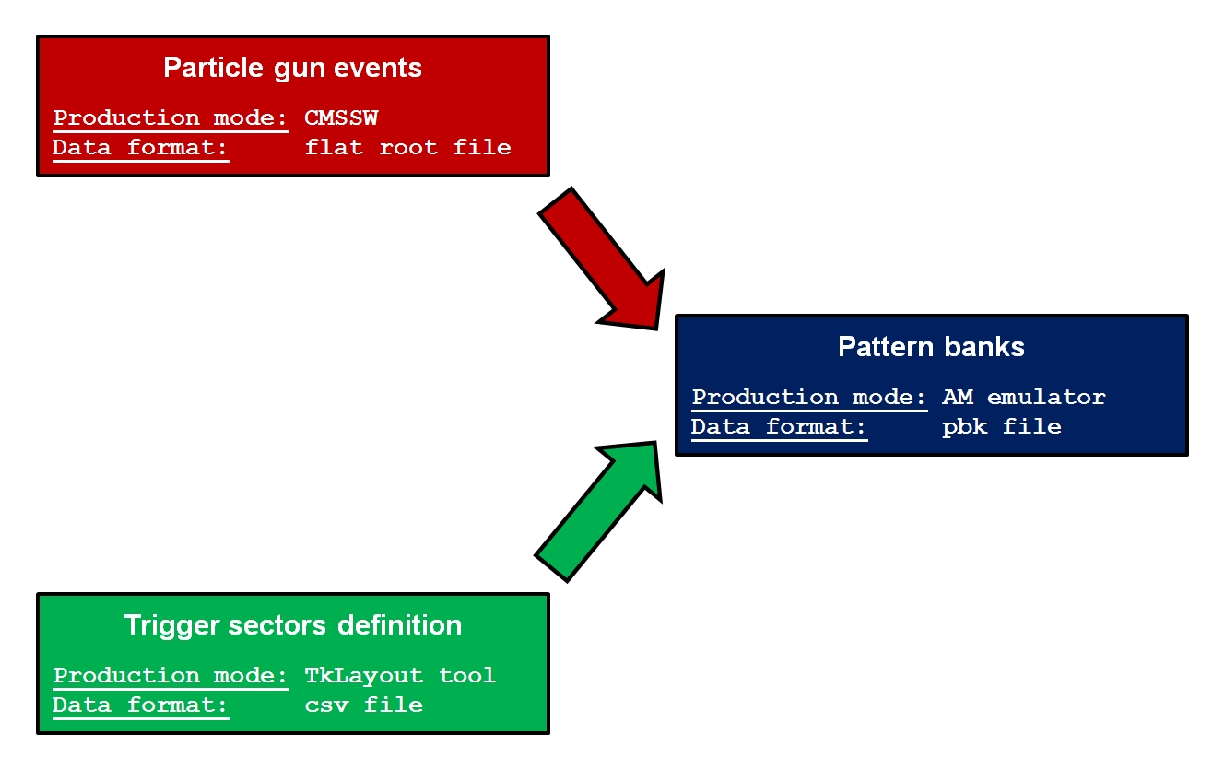
\includegraphics[width=0.6\columnwidth]{Plots/BankGen.eps}
\caption{Pattern bank generation principle}
\label{fig:BkGen}
\end{figure}

\noindent Based on these inputs, the code is able to generate a pattern bank for a given trigger tower. Bank parameters can be set in the configuration file of the bank generation job. In particular, AM chip specific mechanism such as don't care (DC) bits have been implemented. The bank generation data-flow is summarized on Fig.~\ref{fig:BkGenDet}.

\begin{figure}[ht!]
\centering
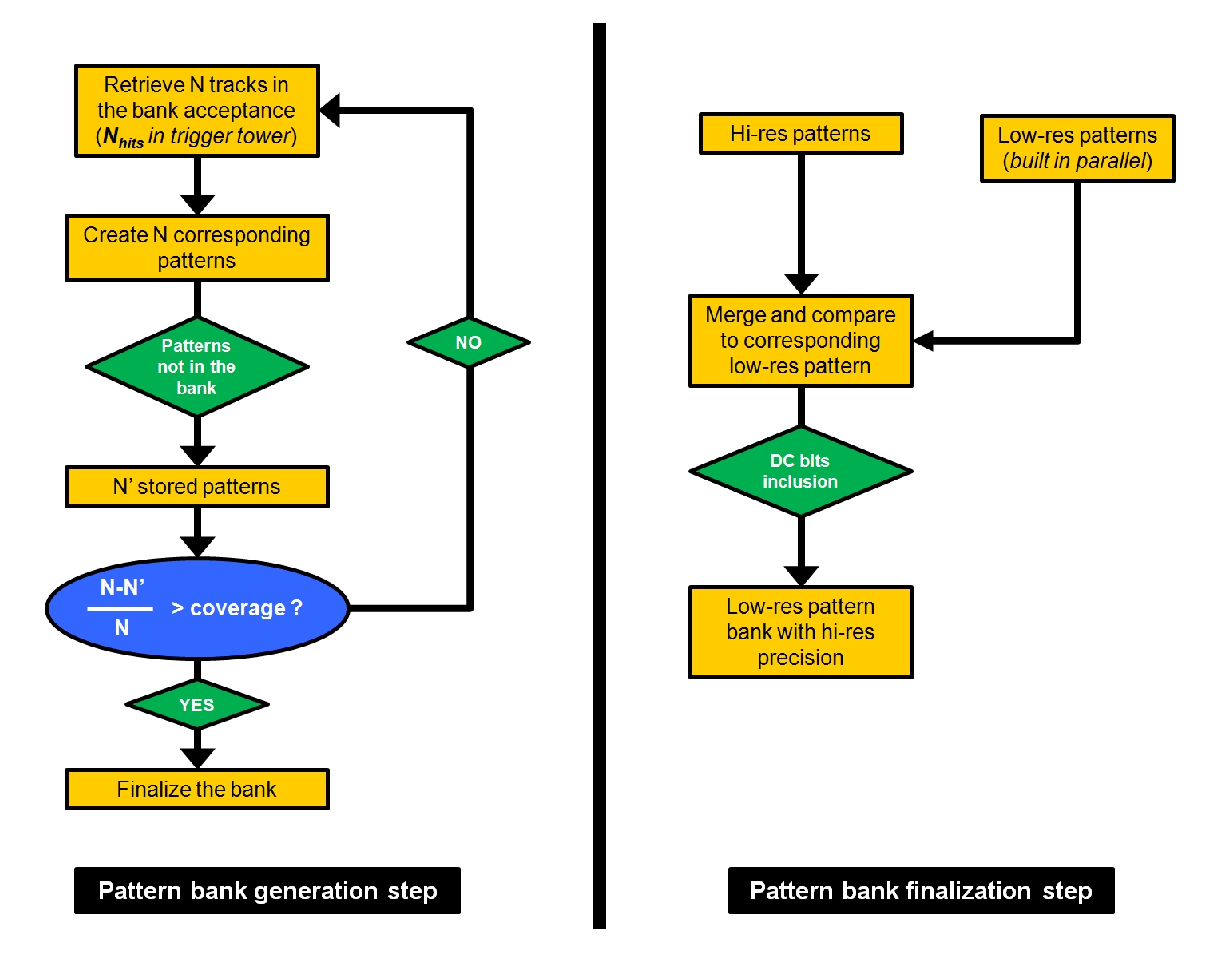
\includegraphics[width=0.6\columnwidth]{Plots/BankGenDetail.eps}
\caption{Pattern bank generation workflow: from track sample to pattern bank}
\label{fig:BkGen}
\end{figure}

\noindent The flow can be divided into two steps: the bank production and the bank finalization. As shown on the left diagram, the bank production is done iteratively. An iteration starts with the collection of tracks satisfying the pattern bank acceptance requirements in the input data sample. This acceptance requirement is defined by the parameter $N_{hits}$, which corresponds to the number of different layer/disks in which the particle has induced a stub in the trigger tower considered. This number should not be confused with the total number of stubs induced by the particle.

\noindent A track will be used to produce a pattern only if $N_{hits}+1$ is larger of equal to the pattern size (we accept the possibility of having one missing hit on the track). In this case, a pattern corresponding to the track is created and stored in the bank if not already in. Iteration ends when a sufficient number of tracks have been collected. At this point, the proportion of tracks collected which were already in the bank is computed. If this proportion is larger than the coverage initially requires, the iteration stage stops.

\noindent Once the required coverage has been reached, the bank is finalized. The procedure is described in the right part of Fig.~\ref{fig:BkGenDet}. At this point two banks have been built. Indeed, every pattern added to the bank produced at the iteration process is linked to a mother pattern of lower resolution. The resolution of this mother pattern is direclty related to the number of DC bits added, the width of the low-res roads is indeed $2^{N_{DC}}$ larger than for the initially built roads. For example, if one requires 2 DC bits, and built pattern with a superstrip size of 32 strips, the width of the low resolution patterns will be 128 strips. 

\noindent At the end of the iterative procedure, each low-res patterns is linked to a set of hi-res patterns. Before storing the low-res pattern in the banks, hi-res patterns belonging to it are merged. The merging result is then compared to the low-res pattern, and the hi-res granularity is kept whenever possible. On the other hand, if all the super-strips are used in a given layer, corresponding DC bits are applied.

\noindent The main advantage of the DC bits procedure is to get high-resolution precision for the price of a low resolution bank. 


\subsection{Pattern recognition}

\subsubsection{Software principle}

\subsubsection{Estimation of the pattern recognition efficiencies and fake rates}


\noindent The generation of the patterns bank is done using a Monte Carlo samples of particle gun $\mu^{\pm}$ produced within the following phase space:
\begin{itemize}
\item $0 < \eta_0 < 2.2$.
\item $1.95GeV/c < p_{T_0} < 100GeV/c$, generated randomly in $1/p_T$.
\item $-15cm < z_0 < 15cm$.
 \item $-1mm < d_0 < 1mm$.
\end{itemize}  

\noindent The direction of the transverse impulsion ($\phi_0$) is chosen such that the generated particles cover the sector we are interested in. The generation procedure is iterative and is using only tracks containing exactly one stub per layer/disk. At iteration $n$, a set of $N$ such tracks is collected. Then one computes the PR efficiency for those tracks using the pattern bank obtained at the end of iteration $n-1$. If the efficiency is larger than a given threshold (called the coverage), the procedure stops. Otherwise, the new patterns formed with those tracks are added to the bank and iteration $n+1$ is done. 

\noindent At the beginning of the first iteration, the bank being empty, every particle will lead to a new pattern insertion. Then, as the bank is being populated, the efficiency growth will become slower.

\subsubsection{Bank efficiency definition}

\noindent Let's denote $N$ the number of tracks you want to reconstruct in a given event, ie the tracks which are within the L1 track trigger requirements. Then, we denote $N^{matched}$ the number of tracks which are contained into at least one pattern. The PR efficiency $\epsilon$ can thus be defined as: 
\begin{equation}
\epsilon = \frac{N^{matched}}{N}
\end{equation} 

\noindent Then, we note $N_{pattern}$ the total number of patterns activated in the event and $N^{matching}_{pattern}$ the number of patterns containing one of the tracks we are looking for. From there one could define the fake rate $\rho$:
\begin{equation}
\rho = 1 - \frac{N^{matching}_{pattern}}{N_{pattern}}
\end{equation} 

\noindent Another important figure is the redundancy $r$. It corresponds to the average number of patterns activated by a good track. 

\noindent Last but not least, one should keep in mind that the PR goal is to provide low-sized hit sets for the track fitting (TF) stage in order to reduce the combinatorics, and consequently the TF time budget. The proportion of good hits per pattern, noted $\epsilon_{hits}$ is therefore a very important parameter:
\begin{equation}
\epsilon_{hits} = \frac{1}{N_{pattern}}\sum_{N_{pattern}}\frac{N_{hits}^{good}}{N_{hits}}
\end{equation} 

\noindent The ideal pattern bank is the one for which:  
\begin{enumerate}
\item $\epsilon = 1$.
\item $\rho = 0$.
\item $r = 1$.
\item $\epsilon_{hits} = 1$. 
\end{enumerate}  

\noindent This ideal bank exists, this is the one for which each possible track in the detector corresponds to one pattern. However, the size of such bank is clearly prohibitive. On the other side, one could imagine the simplest bank with 1 single pattern defined by the whole detector. Such a bank will have $\epsilon=1$, $\rho = 0$ and $r = 1$, but $\epsilon_{hits}$ will be close to 0. Such a solution would be highly inefficient, as TF would be impossible to process. Therefore the optimal solution lies in between, and one realizes that a parameter will be very important: the size of the patterns. The patterns will have to be sufficiently small in order to get a reasonable $\epsilon_{hits}$, but also sufficiently large in order get a reasonable pattern bank size. 


\subsection{Further developments and improvements}


\clearpage
